\documentclass[acmlarge]{acmart}


\AtBeginDocument{%
  \providecommand\BibTeX{{%
    Bib\TeX}}}
  \settopmatter{printacmref=false}

\renewcommand{\descriptionlabel}[1]{\hspace{\labelsep}\textit{#1}}
\usepackage{xcolor}
\newcommand{\todo}{{\color{red}\textbf{TODO} }}
\newcommand{\disease}{{\small \texttt{DISEASE}} }
\newcommand{\hospital}{{\small \texttt{HOSPITAL}} }
\newcommand{\storage}{{\small \texttt{STORAGE}} }

% christos 1, 4
% vasilis 2, 3

\usepackage{amsmath}
\usepackage{subfig}

\begin{document}

\title{Multi-Threading Programming and Inter-Process Communication}
\subtitle{M.Sc. course on ``Technologies for Big Data Analysis'' - Assignment 1}

\author{Christos Balaktsis (1234)}
\email{balaktsis@csd.auth.gr}
\author{Vasileios Papastergios (1234)}
\email{papster@csd.auth.gr}
\affiliation{
  \institution{Aristotle University}
  \city{Thessaloniki}
  \country{Greece}
}

\renewcommand{\shortauthors}{C. Balaktsis and V. Papastergios}
\maketitle

\section{Introduction}

The current document is a technical report for the first programming assignment in the M.Sc. course on \emph{Technologies for Big Data Analysis}, offered by the \emph{DWS M.Sc Program}\footnote{https://dws.csd.auth.gr/} of the Aristotle University of Thessaloniki, Greece. The course is taught by Professor Apostolos Papadopoulos~\footnote{https://datalab-old.csd.auth.gr/$\sim$apostol/}. The authors attended the course during their first year of Ph.D. studies at the Institution.

The assignment contains 4 sub-problems and is part of a series, comprising 3 programming assignments on the following topics:
\begin{description}
  \item[Assignment 1] Multi-threading Programming and Inter-Process Communication
  \item[Assignment 2] The Map-Reduce Programming Paradigm
  \item[Assignment 3] Big Data Analytics with Scala and Apache Spark
\end{description}
In this document we focus on Assignment 1 and its 4 sub-problems. We refer to them as \emph{problems} in the rest of the document for simplicity. The source code of our solution has been made available at \texttt{\small https://github.com/ Bilpapster/big-data-playground}.

\textbf{Roadmap}.
The rest of our work is structured as follows. We devote one section for each one of the 4 problems. That means problems 1, 2, 3 and 4 are presented in sections \ref{section:problem1}, \ref{section:problem2}, \ref{section:problem3} and \ref{section:problem4} respectively. For each problem, we first provide the problem statement, as given by the assignment. Next, we thoroughly present the reasoning and/or methodology we have adopted to approach the problem and devise a solution. Wherever applicable, we also provide insights about the source code implementation we have developed. For problems 2 and 4, we complete the respective sections with a discussion about alternatives or improvements the solution could accept, in order to successfully support more complex requirements. Finally, we conclude our work in section \ref{section:conclusion}.

\section{Problem 1: Concurrent Array-Vector Multiplication}
\label{section:problem1}
We discuss here the first problem of the assignment. The main target of the assignment is using multi-threading programming in Java programming language to concurrently perform an algebraic operation.
\subsection{Problem Statement}
It is known that in Linear Algebra we can multiply a matrix with a vector from the right-hand side, provided that the number of columns in the matrix equals the number of rows in the vector. For instance, given a matrix $\mathbf{A}$ with dimensions $n~\times~m$ and a vector $v$ with dimensions $m~\times~1$, then the product $\mathbf{A}*\mathbf{v}$ is an $n~\times~1$ vector, which results from the implementation of the well-known method of multiplying a matrix with a vector. An example is given following:
\begin{displaymath}
  \begin{bmatrix}
    1 & 0 & 2 & 0 \\
    0 & 3 & 0 & 4 \\
    0 & 0 & 5 & 0 \\
    6 & 0 & 0 & 7
  \end{bmatrix}
  \cdot
  \begin{bmatrix}
    2 \\
    5 \\
    1 \\
    8
  \end{bmatrix}
  =
  \begin{bmatrix}
    4  \\
    47 \\
    5  \\
    68
  \end{bmatrix}
\end{displaymath}

Provided that we are capable of using $k$ threads, where $k$ is a power of 2 and the matrix has dimensions $n~\times~m$, where $n$ is also a power of 2 and $n>k$, design a solution that computes the product $\mathbf{A}*\mathbf{v}$ using $k$ threads with the most efficient way. Your solution has to initialize both the matrix $\mathbf{A}$ and the vector $\mathbf{v}$ with random numbers in the range $[0, 10]$.

\subsection{Proposed approach}

\subsubsection{Setting}
Our implementation is run and tested in a Linux environment, using the Java programming language. We have used the Java Development Kit (JDK) version 11.0.11. The source code is developed in IntelliJ IDEA Community Edition 2021.1.1. The code is compiled and executed in the terminal, using the following commands, starting from the root folder of the repository:
\begin{verbatim}
  cd MatrixMultiplication
  javac MatrixMultiplier.java <n> <m> <k>
  java MatrixMultiplier
\end{verbatim}

\subsubsection{Implementation}
The implementation of the solution proceeds as follows.

First, the main thread initializes the matrix $\mathbf{A}$, of size $n \times m$, and the vector $\mathbf{v}$, of size $n \times 1$, with random numbers in the range $[0, 10]$. Next, the main thread creates $k$ threads, where $k$ is a power of 2. All threads are initiated with references to the matrix $\mathbf{A}$, the vector $\mathbf{v}$, and an empty vector $\mathbf{result}$. The latter is used to store the result of the product of the assigned rows of the matrix with the vector.

Each thread is assigned a range of rows of the matrix $\mathbf{A}$, determined by the $start$ and $end$ indices, to process. The range is calculated based on the total number of rows and the number of threads, i.e., $\lfloor n/k \rfloor$, with the last thread being assigned any remaining rows, covering cases off the assumption that $n,k$ are powers of 2. Each thread then computes the product of the assigned rows of the matrix $\mathbf{A}$ with the vector $\mathbf{v}$ by iterating over the assigned rows and multiplying the corresponding row of the matrix with the vector. It is worth noting that although the thread retains access to the whole matrix, it only accesses the indicated rows. Finally, the result of this computation is stored in the corresponding indices of the vector $\mathbf{result}$, which is shared among all threads, so it is filled concurrently.

Once all threads have completed their assigned computations, the main thread waits for them to finish. It then collects the results from all the threads and prints the final result. In the end, the main thread also prints the total time taken to compute the whole product, which is the time taken for all the threads to finish their computations, excluding the time taken for the initializations of the structures and threads.


\section{Problem 2: Race against a pandemic}
\label{section:problem2}
The second problem asks for leveraging multi-threading programming in Java programming language, in order to simulate a pandemic spread.
\subsection{Problem Statement}
In this problem, you have to simulate a (simplified) pandemic spread, taking into account new infections, hospitalizations and recoveries occurring concurrently. In particular, suppose that a thread named \disease produces periodically (e.g., every 1 second) a random number of new infected people in the range $(0, k]$ that are in need of hospitalization in ICU\footnote{ICU: Intensive Care Unit}. The Health Care System has a limited number of ICU beds, let $e$ (e.g., 20). At the same time, a thread named \hospital periodically (e.g., every 5 seconds) treats a random number of infected patients in the range $(0, h]$, where $h<k$. When a patient is treated the ICU bed used for their treatment is no longer occupied; thus available for use by another patient.

Develop a solution that simulates the above behavior. Your solution should also keep track of the total number of treated patients, as well as the ones that were not able to find a spot in ICU. The simulation must complete its execution after a predefined number of steps (or time period), which will be given as program argument, alongside with all aforementioned parameters (periods, $k$, $h$, $e$). You should test your solution against different values of the parameters, in order to verify that it correctly operates in all possible cases. How would you convert your solution if, instead of a single hospital, there were three of them, with a single, shared queue of patients?

\subsection{Proposed approach}

\subsubsection{Setting}
Our implementation is run and tested in both a Linux (Ubuntu 24.04) and a Windows 11 environment, using the Java programming language. We have used JDK 11.0.11 and IntelliJ IDEA Community Edition 2021.1.1. The code is compiled and executed in the terminal, using the following commands, starting from the root folder of the repository:

\begin{verbatim}
  cd raceAgainstPandemic
  javac RaceAgainstPandemic.java <dur> <beds> <d_per> <inf> <h_per> <tr>
  java RaceAgainstPandemic
\end{verbatim}
where:
\begin{itemize}
  \item \texttt{<dur>} is the total duration to run the simulation
  \item \texttt{<beds>} is the total number of available ICU beds
  \item \texttt{<d\_per>} is the time period between two infection steps
  \item \texttt{<inf>} is the maximum number of infections per step
  \item \texttt{<h\_per>} is the time period between two treatment steps
  \item \texttt{<tr>} is the maximum number of treatments per step
\end{itemize}
Note that the command line arguments have to be exactly 6 and all individual arguments should be integer parsable. An exception will be thrown, in case any of the aforementioned conditions is violated, accompanied by an explanatory message.

\subsubsection{Implementation}
We develop our solution on top of two custom-defined classes, namely \texttt{Disease} and \texttt{Hospital}. Both classes are defined as subclasses of the Java's \texttt{Thread} class. We encapsulate the logic of the two classes in the overridden \texttt{run()}. In particular,
\begin{itemize}
  \item The \texttt{Disease} thread repeats two actions: (1) creates a new number of infections and then (2) sleeps for \texttt{<d\_per>} seconds.
  \item The \texttt{hospital} thread follows the same scheme, with the difference that it populates new treatments, instead of infections.
\end{itemize}

The communication of these two threads is accomplished via a third, custom-defined Java class, namely \texttt{HealthCareManager}. We implement this class employing the \textit{Singleton} design pattern, to ensure that only one instance of this class will be created at runtime and this instance will be shared among all running threads. Inside this class, we encapsulate the logic of handling new infections and treatments when they occur by the \texttt{Disease} and \texttt{Hospital} threads respectively. The \textbf{key functionality} of the \texttt{HealthCareManager} class is to ensure \textbf{synchronization and mutual exclusion} between the two threads, when the counters are accessed and modified. The critical counters the \texttt{HealthCareManager} instance updates are the following:
\begin{itemize}
  \item \texttt{totalBeds}: the total number of ICU beds in the Health Care System
  \item \texttt{availableBeds}: the number of currently available ICU beds
  \item \texttt{currentlyInICU}: the number of patients \emph{currently} in ICU
  \item \texttt{currentlyOutOfICU}: the number of patients \emph{currently} waiting for ICU treatment (out of ICU)
  \item \texttt{totalTreatments}: the total number of patients treated from the start of the simulation up to that moment
  \item \texttt{totalInfections}: the total number of people infected from the start of the simulation up to that moment
\end{itemize}

We refer to these counters as \emph{critical}, since both threads are competing for accessing and updating them in a contradictory way. In particular, the \texttt{Disease} thread produces new infections, increasing \texttt{totalInfections} and possibly \texttt{currentlyInICU}, \texttt{currentlyOutOfICU}, while possibly decreasing \texttt{availableBeds}. The \texttt{Hospital} thread, on the other hand, produces new treatments with the completely opposite effects.

In order to ensure that the counters are accessed and updated consistently by the two threads, we extract all updates to a dedicated, \texttt{synchronized} method, inside the \texttt{HealthCareManager}. We note that, when the Java keyword \texttt{synchronized} is used in a method, Java ensures that \textbf{exactly one} thread can have access to this method, while all others competing for it are locked out (waiting), until the former thread exits the method. We refer the interested reader to the \texttt{handleUpdate()} method of the \texttt{HealthCareManager} class for the exact implementation.

\subsubsection{Testing thread-safety}

We discuss here the methodology we have adopted to test the thread-safety property of our implementation. We implement our testing methodology on top of the following property that derives from the problem statement:
\begin{description}
  \item[Property] The patients in ICU, the patients waiting for (i.e., out of) ICU and the total number of treated people must add up to the total number of infections. The property is formally expressed in equation~\ref{equation:thread_safety_property_pandemic}.
\end{description}
\begin{equation}
  \label{equation:thread_safety_property_pandemic}
  \text{currentlyInICU}_t + \text{currentlyOutOfICU}_t + \text{totalTreatments}_t = \text{totalInfections}_t~\forall~ t \in [t_{start}, t_{end}],
\end{equation}
where $t_{start}$ and $t_{end}$ are the start and end timestamp of the simulation respectively and the subscript $t$ indicates the timestamp that the counters are accessed at.

We leverage this property to test and evaluate the thread safety of our implementation. In order to do so, we have used the Java's \texttt{junit} library for unit testing. More specifically, we define a test case where a simulation is run. The counters are accessed at the end of the simulation, checking whether the aforementioned property holds. To strengthen our experimental testing, we opt for executing the test 10 times with random initial configurations each time. A snapshot of the test results is depicted in figure~\ref{img:thread_safety_tests}, where all 10 runs of the simulation (with random initial configurations each) are successfully passed (i.e., equation~\ref{equation:thread_safety_property_pandemic} holds at the end of all simulations). We refer the interested reader to the \texttt{test/TestRaceAgainstPandemic.java} file for more details about the implementation of the unit test.

\begin{figure}[tb]
  \centering
  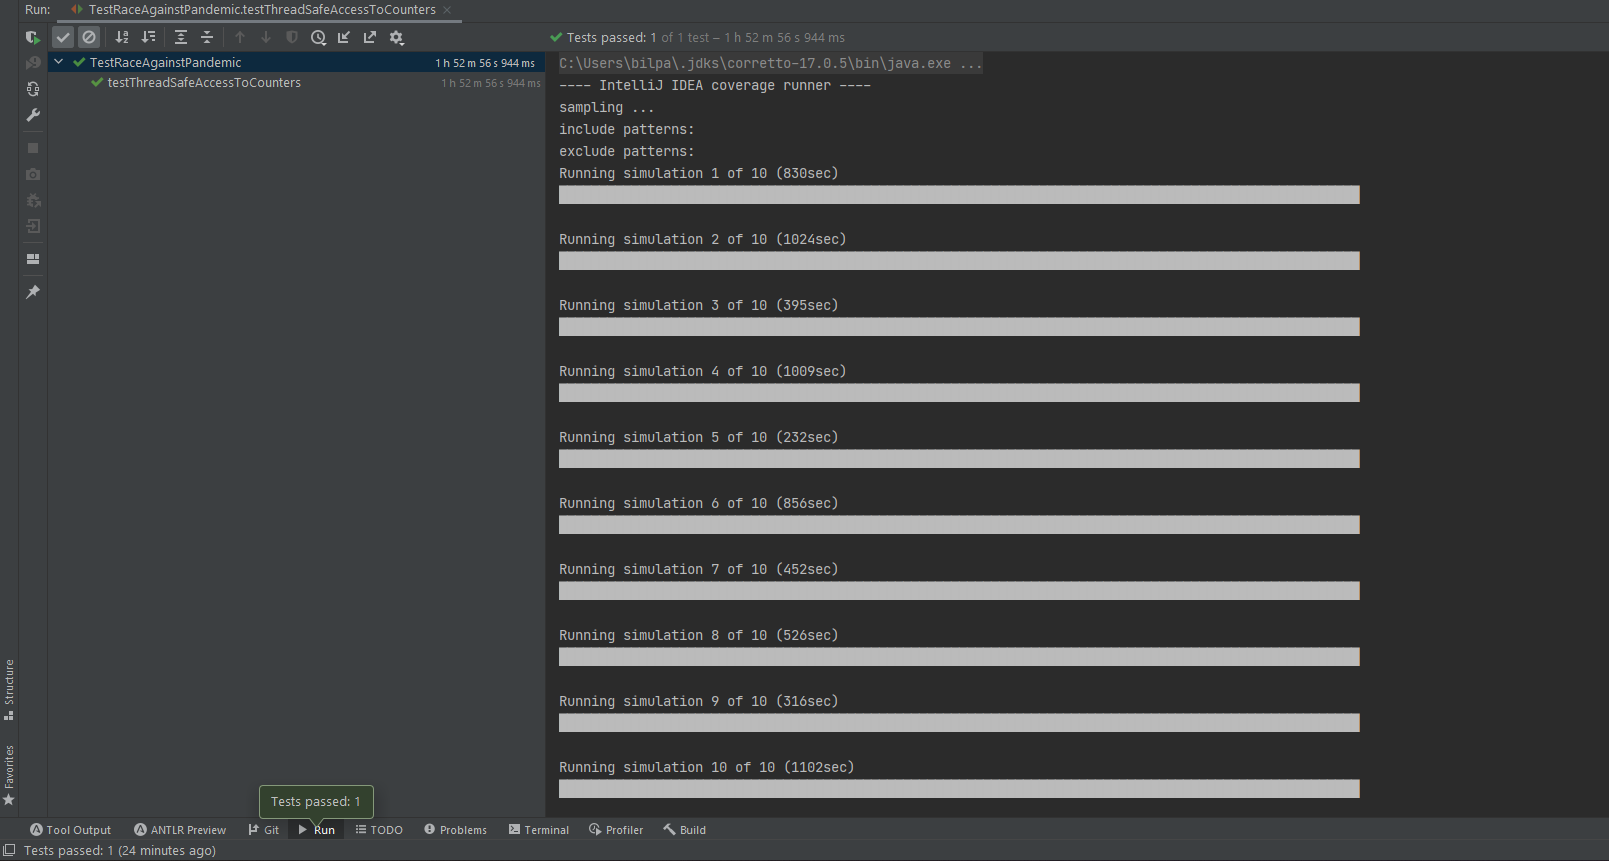
\includegraphics[width=0.75\linewidth]{figures/thread safety testing.png}
  \caption{Test results for thread-safety. Ten simulations are run with random initial configurations and equation~\ref{equation:thread_safety_property_pandemic} is tested at each simulation end. All tests are successfully passed.}
  \Description{A snapshot from IntelliJ IDEA testing environment.}
  \label{img:thread_safety_tests}
\end{figure}

\subsubsection{Screenshots and Visualizations}
In this subsection we briefly present execution screenshots and visualizations of the simulation. In particular, figure~\ref{img:disease_hospital_execution} shows the execution of a simulation inside IntelliJ IDEA. The program prints the simulation configurations and shows a progress bar during the simulation run. When the simulation is over, the program outputs the counter values.

\begin{figure}[h]
  \centering
  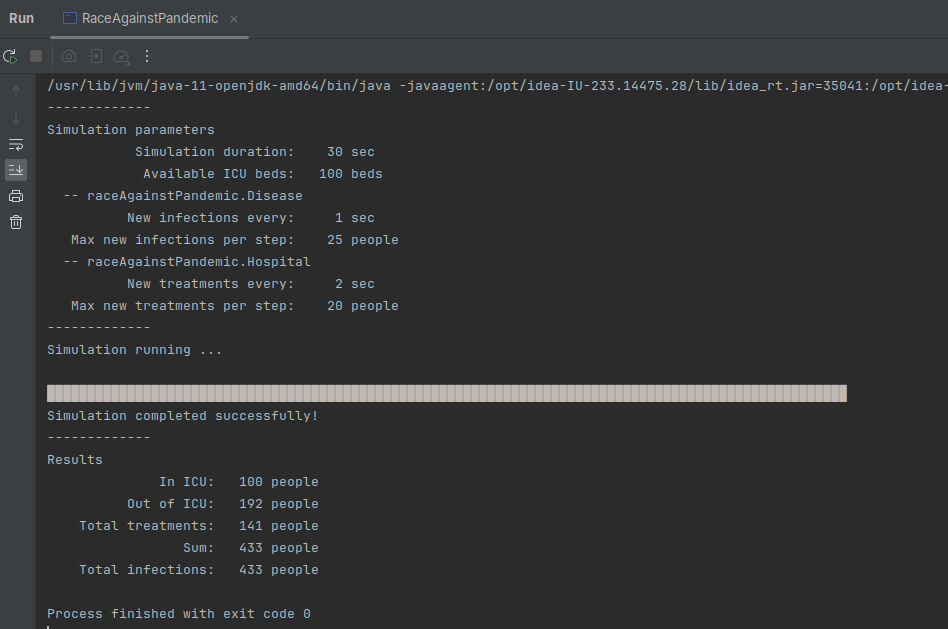
\includegraphics[width=0.75\linewidth]{figures/disease-hospital-execution.png}
  \caption{Execution of a simulation inside IntelliJ IDEA.}
  \Description{A snapshot from IntelliJ IDEA testing environment.}
  \label{img:disease_hospital_execution}
\end{figure}

Concerning visualizations, figure~\ref{img:disease_hospital_visualizations}a depicts the number of patients in and out of ICU over time for a single simulation with duration of 10 minutes and 100 available ICU beds in total. Figure~\ref{img:disease_hospital_visualizations}b shows the cumulative number of infections and treatments over time for the same setting.

\begin{figure}[h]
  \centering
  \subfloat[Number of patients in (orange) and out of ICU (red) \\ over time]{
    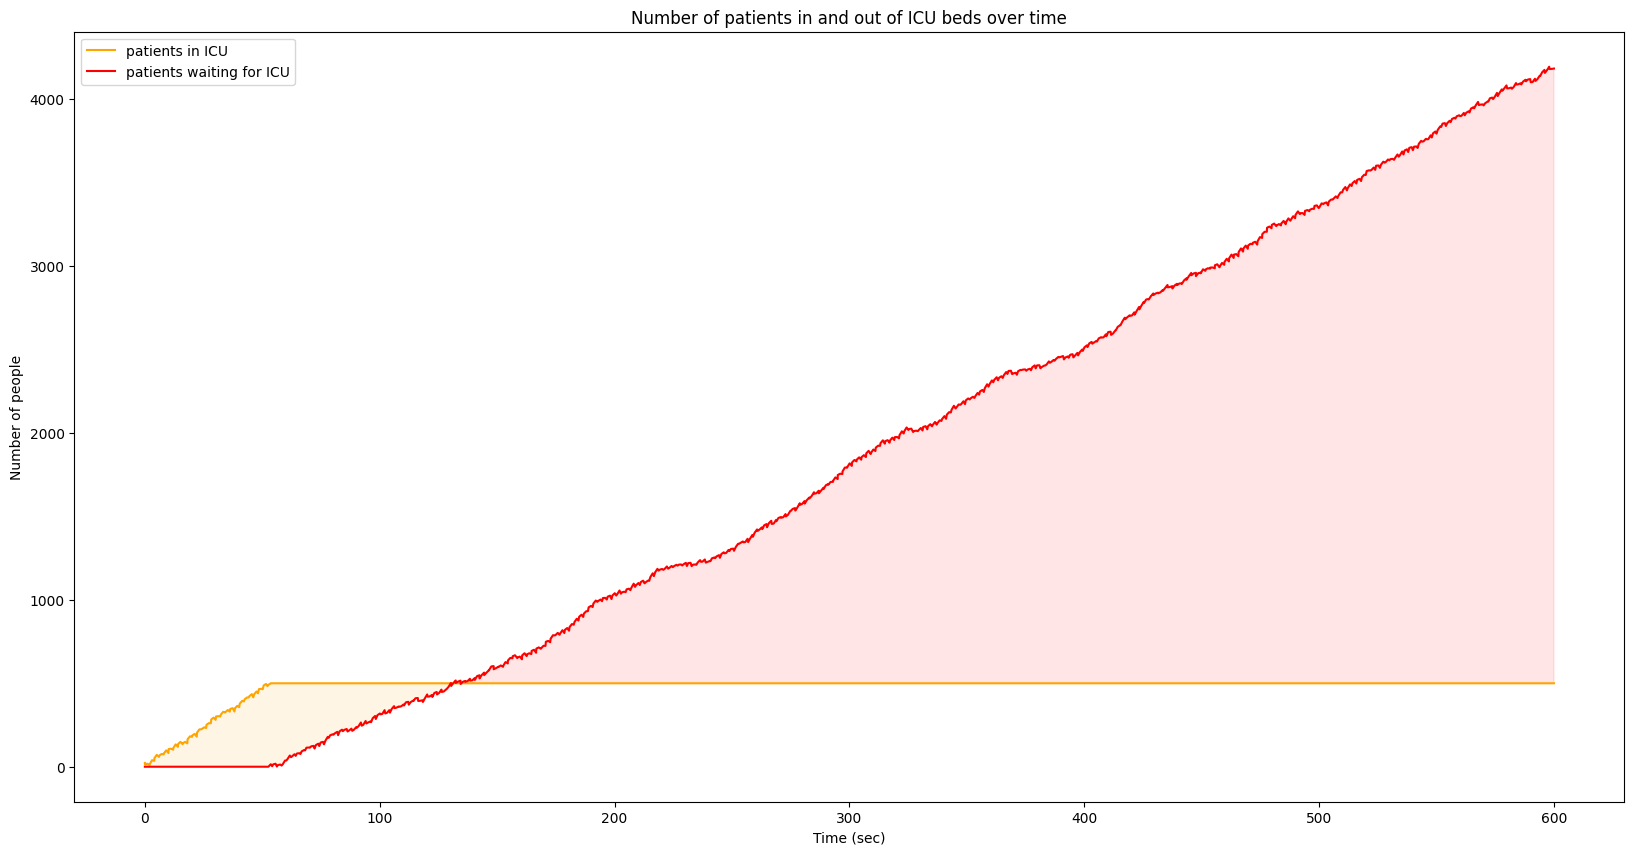
\includegraphics[width=.5\linewidth]{figures/in-out ICU.png}
  }
  \subfloat[Cumulative treatments (green) and infections (red) over time]{
    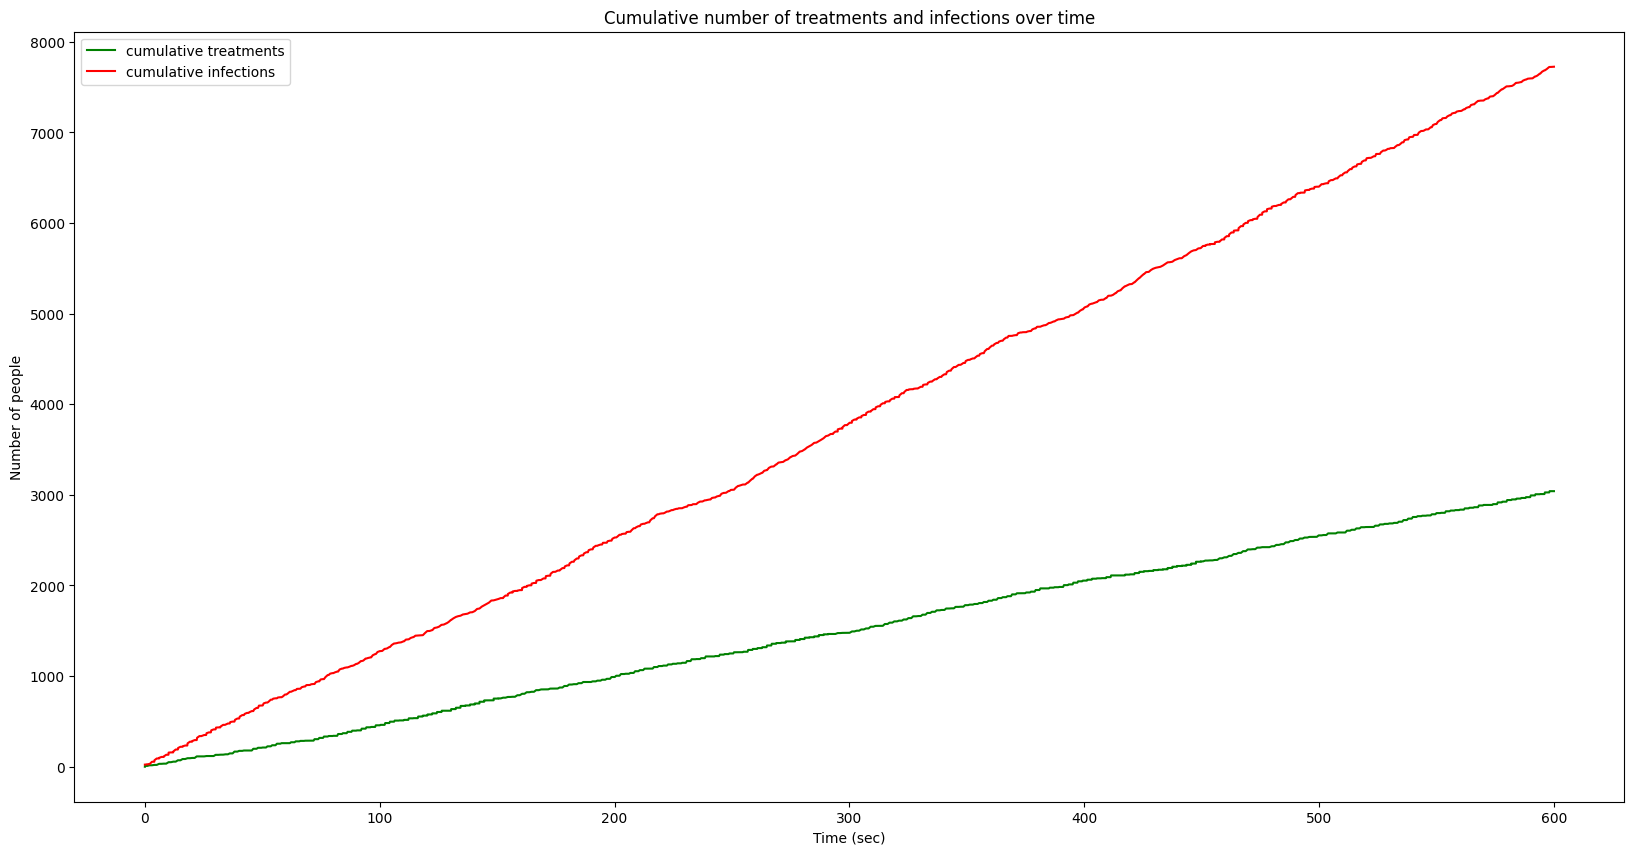
\includegraphics[width=.5\linewidth]{figures/treatments-infections.png}
  }
  \caption{Visualizations for a single 10-minute simulation with 100 available ICU beds, at most 25 new infections every 1 second and at most 20 new treatments every 2 seconds.}
  \label{img:disease_hospital_visualizations}
\end{figure}



\subsubsection{Limitations of current implementation and further improvements}
The current implementation successfully addresses the \disease - \hospital problem when \emph{exactly one} thread of both entities are active every time moment. This means there is only one \disease thread that periodically produces new infections and only one \hospital thread that periodically treats some of them. We can imagine the new infections and treatments at every step as a sequence of requests, which are handled by the Health Care System. The latter lives in the main thread of our application. Thanks to the use of the \texttt{synchronized} Java keyword, the Health Care System is able to handle the requests as if they were put in an imaginary \textbf{single queue}, where only one request is processed at a time and the inner critical counters are accessed and modified consistently.

A more generic version of the problem could contain multiple \disease and multiple \hospital threads running at the same time, each one of them producing a random, independent number of new infections and treatments respectively. In such a case, the Health Care System handles again all produced requests as if they were put in a single queue, where only one request modifies the critical counters at a time. \textbf{We claim that our implementation can successfully handle this generic version of the problem} with trivial changes. The only requirement for our implementation to work properly in such a scenario is that all running \disease and \hospital threads are provided with the same instance of the \texttt{HealthCareManager} class. This requirement holds, since we have implemented the class using the \textbf{Singleton} design pattern, ensuring that it can be instantiated only once and all other objects share this instance.

Apart from this requirement, only few trivial changes need to be made. In particular, more \texttt{Disease} and \texttt{Hospital} instances should be created, meeting the needs of the generic problem statement. The mutual exclusion ensured by the \texttt{synchronized} character of the processing method simulates the handling of requests as if they were in a single queue. \textbf{We verify our claim by executing unit tests with multiple \disease and multiple \hospital threads running at the same time}. We run 10 test simulations with random initial configurations each. All tests are successfully passed. The tests' implementation can be found in \texttt{test/TestRaceAgainstPandemic.java} file and, in particular, in \texttt{testMultiDiseaseMultiHospitalVersion()} method. 


\section{Problem 3: Key-value server store}
\label{section:problem3}
We present here the third problem of the assignment. The main focus of the problem is the inter-process communication, leveraging TCP sockets in Java programming language.

\subsection{Problem Statement}
Develop a client-server application that works as follows.

\textbf{Server}. The server starts its operation by initializing an empty Hash Table. The Hash Table stores key-value pairs and has size of $2^{20}$. Next, the server opens a TCP port, the number of which is passed as a program argument (e.g., 8888, 9999, etc.). The server awaits for clients to connect.

\textbf{Client}. The client starts its operation by trying to connect with the server, in the specified TCP port. Again, the port is passed as a program argument.

\textbf{Communication protocol}. After the successful connection between server and client, the client can send messages to the server, requesting some action from a predefined list of available actions. In particular, the client can perform the following operations:
\begin{description}
  \item[Operation 0] Terminates the connection between client and server. Operation code: \texttt{0}.
  \item[Operation 1] Inserts a key-value pair in the Hash Table stored in the server-side. Operation code: (\texttt{1, K, V}), where \texttt{K} and \texttt{V} is the key and value to be inserted respectively.
  \item[Operation 2] Deletes a key-value pair from the Hash Table kept in the server-side. Operation code: (\texttt{2, K}), where \texttt{K} is the key to be deleted, jointly with the stored value that is associated with it.
  \item[Operation 3] Searches for a key and retrieves its value (if exists). Operation code: (\texttt{3, K}), where \texttt{K} is the key to search for.
\end{description}


\section{Problem 4: Multi-server producer-consumer interaction}
\label{section:problem4}
The fourth problem of the assignment concerns a more complex scenario of inter-process communication with multiple servers being active simultaneously. The assignment asks for implementation in Java programming language, leveraging TCP sockets and multi-threading.
\subsection{Problem Statement}
Suppose that you want to develop a process system that consists of three types of processes: \textbf{consume}, \textbf{produce} and \textbf{server}. All three types of processes communicate with each other using TCP sockets. The system operation is as follows.

\textbf{Server}. Each server has a non-shared integer variable \storage that depicts the quantity of products in stock, located in the specific server. The initial value of the \storage for each server is a random integer number in the range $[0, 100]$.

\textbf{Producer}. Each producer connects randomly to a server and adds a random value X in the range $[10, 100]$ to the \storage variable of the specific server. In case the new \storage value exceeds 1000, then the respective server sends a message and the value is not updated. Next, the producer awaits for a random period of time in the range $[1, 10]$ seconds and connects to the next server, again randomly.

\textbf{Consumer}. Each consumer randomly connects to a server and subtracts a random value Y in the range $[10, 100]$ from \storage of this server. If the new \storage value is below 1, then the respective server sends a relevant message and the \storage value is not updated. Next, the consumer awaits for a random time period in the range $[1, 10]$ and connects to the next server, again randomly.


\section{Conclusion}
\label{section:conclusion}
This is the section for the conclusion.


\end{document}
\endinput
%%
%% End of file `sample-acmlarge.tex'.
